\documentclass[10pt]{article}
\usepackage[utf8]{inputenc}
\usepackage{graphicx}
\usepackage{amsmath}
\usepackage{amssymb}
\usepackage{geometry}
\usepackage{setspace}
\usepackage{abstract}
\usepackage{titlesec}
\usepackage[backend=biber,style=apa]{biblatex}% Changed style to apa
\usepackage[hidelinks]{hyperref}
\PassOptionsToPackage{hyphens}{url} % Pass hyphens option to url package via hyperref
\usepackage{fancyhdr} % For custom headers and footers
\usepackage{lastpage} % For page numbering in the footer
\usepackage{xcolor} % For text color
\usepackage{tabularx} % Tabularx package for better table formatting
\usepackage{longtable}% Long table package for tables that span multiple pages

% Set marginparwidth for todonotes
\setlength{\marginparwidth}{2cm} % Adjust the marginparwidth
\usepackage{todonotes} % TODOs
\usepackage{tcolorbox} % For colored boxes
\usepackage{caption} % For custom captions

% Fonts and typography
\usepackage{helvet} % Load the Helvetica font package
\renewcommand{\familydefault}{\sfdefault} % Set sans-serif as the default font family

% Page setup
\geometry{margin=1in}
\setstretch{1.2}
\titleformat{\section}{\bfseries\Large}{\thesection}{1em}{}
\titleformat{\subsection}{\bfseries\large}{\thesubsection}{1em}{}
\titleformat{\subsubsection}{\bfseries\normalsize}{\thesubsubsection}{1em}{}

% Add bibliography file
\addbibresource{references.bib}

% Customization to remove url date and format URLs and DOIs
\AtEveryBibitem{%
  \ifentrytype{online}{%
    \clearfield{urldate}%
    \clearfield{note}%
  }{}%
  \ifentrytype{article}{%
    \clearfield{urldate}%
  }{}%
}

\renewbibmacro*{doi+eprint+url}{%
  \printfield{doi}%
  \newunit\newblock%
  \iffieldundef{doi}{%
    \usebibmacro{eprint}%
    \newunit\newblock%
    \usebibmacro{url+urldate}}%
    {}%
}

% Customize the caption format
\captionsetup[figure]{
    labelfont=bf,           % Bold font for the label
    labelsep=space           % Use a space as the separator
}
\captionsetup[table]{
    labelfont=bf,           % Bold font for the label
    labelsep=space           % Use a space as the separator
}

% Change font size of bibliography entries
\renewcommand{\bibfont}{\fontsize{7pt}{9pt}\selectfont}% Set font size to 7pt, maybe too small. Change to 8pt if needed. Also adjust actual text size?

% Title
\title{Visual Cortical Prostheses: Bridging Technology, AI and Human Vision for the Future}
\author{
  Marc J. Posthuma\\
  Student Number: 4413105\\
  \texttt{marc.posthuma@ru.nl}\\
  \\
  Radboud University\\
  Supervisor: dr.\ F.\ Zeldenrust\\
  Department of Neurophysics, Donders Centre for Neuroscience
}
\date{\today}

% Adjust page geometry to balance header and footer
\geometry{
  a4paper,
  left=20mm,
  right=20mm,
  top=30mm,
  bottom=30mm,
  headheight=60.50554pt, % Set the head height
  headsep=10pt, % Space between header and text
  footskip=30pt % Space between text and footer
}

% Custom footrule commands
\newcommand{\blackfootrule}{%
  \color{black}\makebox[\headwidth]{\rule[0.5ex]{\headwidth}{0.3pt}}%
}

\newcommand{\grayfootrule}{%
  \color{gray}\makebox[\headwidth]{\rule[0.5ex]{\headwidth}{0.3pt}}%
}

% Define fancyhdr styles
\fancypagestyle{firstpage}{
  \fancyhf{}
  \fancyhead[L]{
\includegraphics[width=5cm, keepaspectratio]{imgs/RU_logo_NL_cropped.png}}
  \fancyhead[R]{\fontsize{10}{12}\selectfont \textbf{Research Proposal} \\ NWI-BM-RESPROP}
  \fancyfoot[L]{\fontsize{8}{10}\selectfont \textcolor{gray}{Radboud University}}
  \fancyfoot[C]{\fontsize{8}{10}\selectfont \textcolor{gray}{\thepage\ of~\pageref{LastPage}}}
  \fancyfoot[R]{\fontsize{8}{10}\selectfont \textcolor{gray}{July 2024}}
  \renewcommand{\footrulewidth}{0.3pt}
  \renewcommand{\footrule}{\blackfootrule}
}

\fancypagestyle{rest}{
  \fancyhf{}
  \fancyhead[L]{\fontsize{8}{10}\selectfont \textcolor{gray}{Research Proposal}}
  \fancyhead[R]{\fontsize{8}{10}\selectfont \textcolor{gray}{Visual Cortical Prostheses: Bridging Technology, AI and Human Vision for the Future}}
  \fancyfoot[L]{\fontsize{8}{10}\selectfont \textcolor{gray}{Radboud University}}
  \fancyfoot[C]{\fontsize{8}{10}\selectfont \textcolor{gray}{\thepage\ of~\pageref{LastPage}}}
  \fancyfoot[R]{\fontsize{8}{10}\selectfont \textcolor{gray}{July 2024}}
  \renewcommand{\footrulewidth}{0.3pt}
  \renewcommand{\footrule}{\grayfootrule}
}

% Redefine the abstract environment to use "Summary" instead of "Abstract"
\makeatletter
\renewenvironment{abstract}{%
    \if@twocolumn%
      \section*{\abstractname}%
    \else
      \begin{center}%
        {\bfseries \large\abstractname\vspace{-.5em}\vspace{\z@}}%
      \end{center}%
      \quotation\small % Ensures the text is smaller
    \fi}
    {\if@twocolumn\else\endquotation\fi}%
\renewcommand{\abstractname}{Summary}
\makeatother

% Document
\begin{document}

\pagestyle{plain}% Default plain page style for the list of TODOs
\listoftodos% Remove this line before submission
\clearpage%To make sure the todo list is on a separate page without fancyhdr

\newpage% To make sure the todo list is on a separate page without fancyhdr

% Title and abstract
\maketitle
\thispagestyle{firstpage} % Apply first page style after title
\begin{abstract}
  \noindent Visual cortical prostheses represent a revolutionary technology
  within the field of neuroprosthetics, aimed at restoring vision for
  individuals with visual impairments through direct neural interfaces. Recent
  advances have focused on retinal and optic nerve implants; however, these do
  not aid individuals with damage beyond these structures. This proposal
  explores the use of artificial intelligence (AI) and virtual reality (VR) to
  optimize visual cortical prostheses by developing AI algorithms that generate
  and refine phosphene patterns, enabling users to visualize dynamic
  environments in real-time. Expanding upon existing phosphene simulators that
  are limited to static images, this research aims to enhance scene
  simplification and phosphene resolution, improving the quality and accuracy of
  visual representations.

  The research is divided into three phases. The first phase involves developing
  initial AI algorithms for scene simplification and phosphene generation using
  Convolutional Neural Networks (CNNs), alongside setting up the experimental
  infrastructure. A diverse group of 20 participants will navigate VR
  environments to collect data on the effectiveness of these algorithms. The
  second phase advances AI models using CNNs, Generative Adversarial Networks
  (GANs), and Reinforcement Learning (RL), coupled with neurophysiological
  studies such as Visual Evoked Potentials (VEP) and fNIRS to assess the impact
  on visual perception. The final phase conducts extensive experiments with a
  larger participant group to validate the AI systems, aiming for real-world
  application readiness.

  This study aims to significantly enhance the user experience of visual
  prosthetics, potentially transforming the field by enabling accurate, dynamic
  visual representations. If successful, it will pave the way for advanced
  neural interfaces and sensory augmentation devices, improving the quality of
  life for individuals with visual impairments. The research highlights the
  importance of interdisciplinary collaboration in advancing neuroprosthetic
  technology, urging continued innovation at the intersection of neuroscience,
  engineering, and AI.\@
\end{abstract}
\textbf{Keywords:} Simulated  phosphene vision, neuroprosthetics, deep learning models, phosphene patterns, real-time image processing

\pagestyle{rest} % Apply rest page style from here
\clearpage % Ensure a new page for the figure and introduction

\begin{figure*}[ht!]
  \centering
  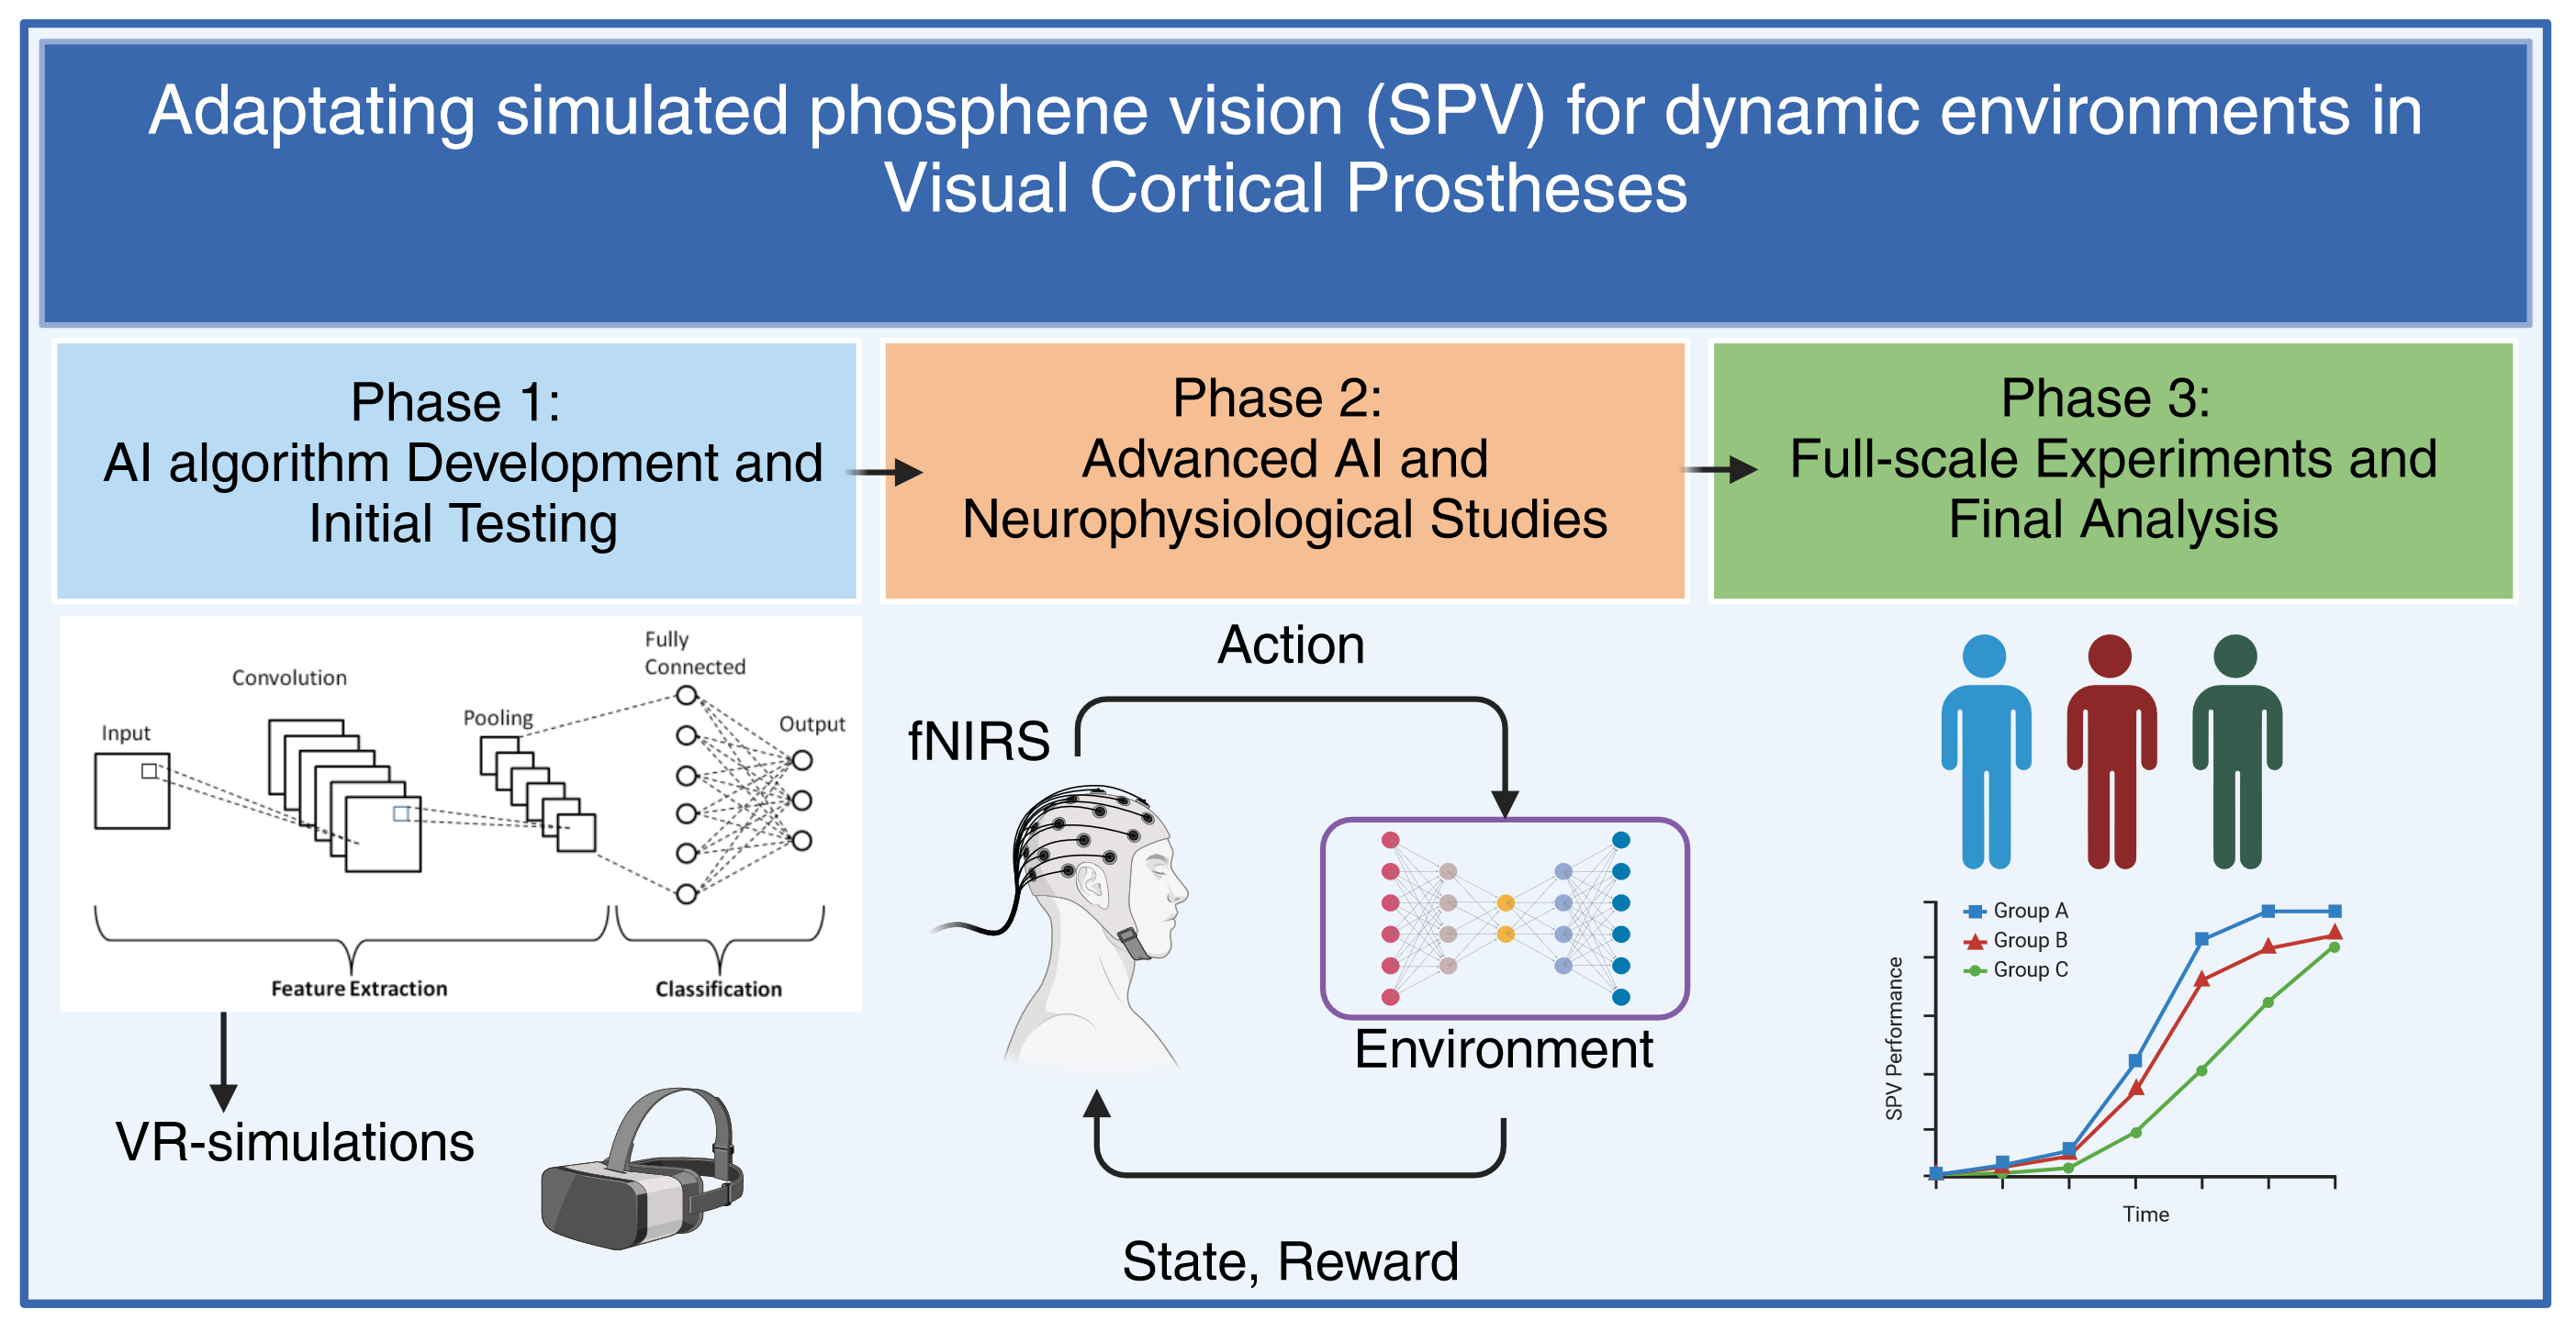
\includegraphics[width=1.0\textwidth]{imgs/SPV_VCP_pipeline.png}
  \caption{| Graphical abstract illustrating the three phases of the research proposal on simulated phosphene vision for visual cortical prostheses: (1) Developing initial AI algorithms for scene simplification and phosphene generation; (2) Advancing AI models with neurophysiological assessments; (3) Conducting extensive experiments for real-world application validation. (Image: BioRender, \href{https://app.biorender.com/}{https://app.biorender.com/}, accessed on 2 July 2024).}\label{fig:graphical_abstract}
\end{figure*}

\section*{Introduction}\label{sec:intro}
Globally, blindness affects millions of people, with estimates rising from over
30 million in 2013 to 43.3 million in
2020~\parencite{stevensGlobalPrevalenceVision2013,bourneTrendsPrevalenceBlindness2021}.
For certain types of blindness, visual prosthetics present a promising avenue
for restoring rudimentary vision through electrical stimulation of the visual
system. In the past decade, significant attempts have already been made in early
systems that focus on retinal and optic nerve implants, such as the exemplary
FDA-approved ARGUSII retinal system by Second Sight
Medical~\parencite{hoLongTermResultsEpiretinal2015}. However, these systems do
not provide a solution for individuals who have damage to structures such as the
retina or optic nerve in the visual pathway.

Visual cortical prostheses provide a novel approach to stimulating the brain by
interface directly with the brain's visual
cortex~\parencite{deruytervansteveninckRealworldIndoorMobility2022}.
These devices convert visual information from the environment into neural
signals that can be processed by the brain.

The core technology involves the generation of phosphenes—perceived spots of
light resulting from electrical stimulation of the visual
cortex~\parencite{vandergrintenBiologicallyPlausiblePhosphene2024}. However,
organizing these phosphenes into coherent and interpretable visual patterns
remains a significant challenge.

In order to optimize these phosphene patterns for more accurate representations
of a user's surroundings, artificial intelligence (AI) can be leveraged in the
form of deep learning algorithms. Algorithms such as Convolutional Neural
Networks (CNNs) have already been proven to be effective for image processing of
static objects in recent work
by~\textcite{deruytervansteveninckEndtoendOptimizationProsthetic2022}. Deep
learning models like CNNs provide a solution to low sampling resolution of
complex visual stimuli, enabling the generation of more detailed and accurate
reconstruction of the visual scene.

The phosphene simulator described in the article
by~\textcite{deruytervansteveninckEndtoendOptimizationProsthetic2022} was
implemented in Python, utilizing the PyTorch deep learning library for its
computational capabilities. It operates by translating electrical stimulation
parameters into an estimated phosphene perception, taking into account the
history of stimulation to ensure accuracy. The simulator initializes with
electrode locations on a flattened cortical map of the primary visual cortex
(V1), using the reverse wedge-dipole visuotopic model to map these locations to
the user's visual field~\parencite{liWearableComputerVision2013}. This model
accounts for the eccentricity and azimuth in the visual field, controlling
various parameters to ensure realistic proportions in cortical distance.

To determine the size of the phosphenes, the simulator uses models that estimate
current spread from the electrodes, incorporating factors like stimulation
current and cortical magnification. The appearance and brightness of phosphenes
are modeled with a sigmoidal activation function, taking into account the
activation threshold, which introduces variability between electrodes. Temporal
dynamics are managed through a memory trace that adjusts phosphene brightness
based on stimulation history, incorporating decay and input effects to simulate
accommodation. Each frame, the simulator processes stimulation parameters,
estimates phosphene characteristics, and renders these effects on a visual field
map, summing them to produce the final simulated prosthetic percept. This
biologically grounded model aims to enhance the realism and efficacy of
simulated prosthetic vision, facilitating the optimization of cortical visual
prosthetic systems. An example of such a framework is shown in Figure~\ref{fig:simulator_framework}.

\begin{figure*}[ht!]
  \centering
  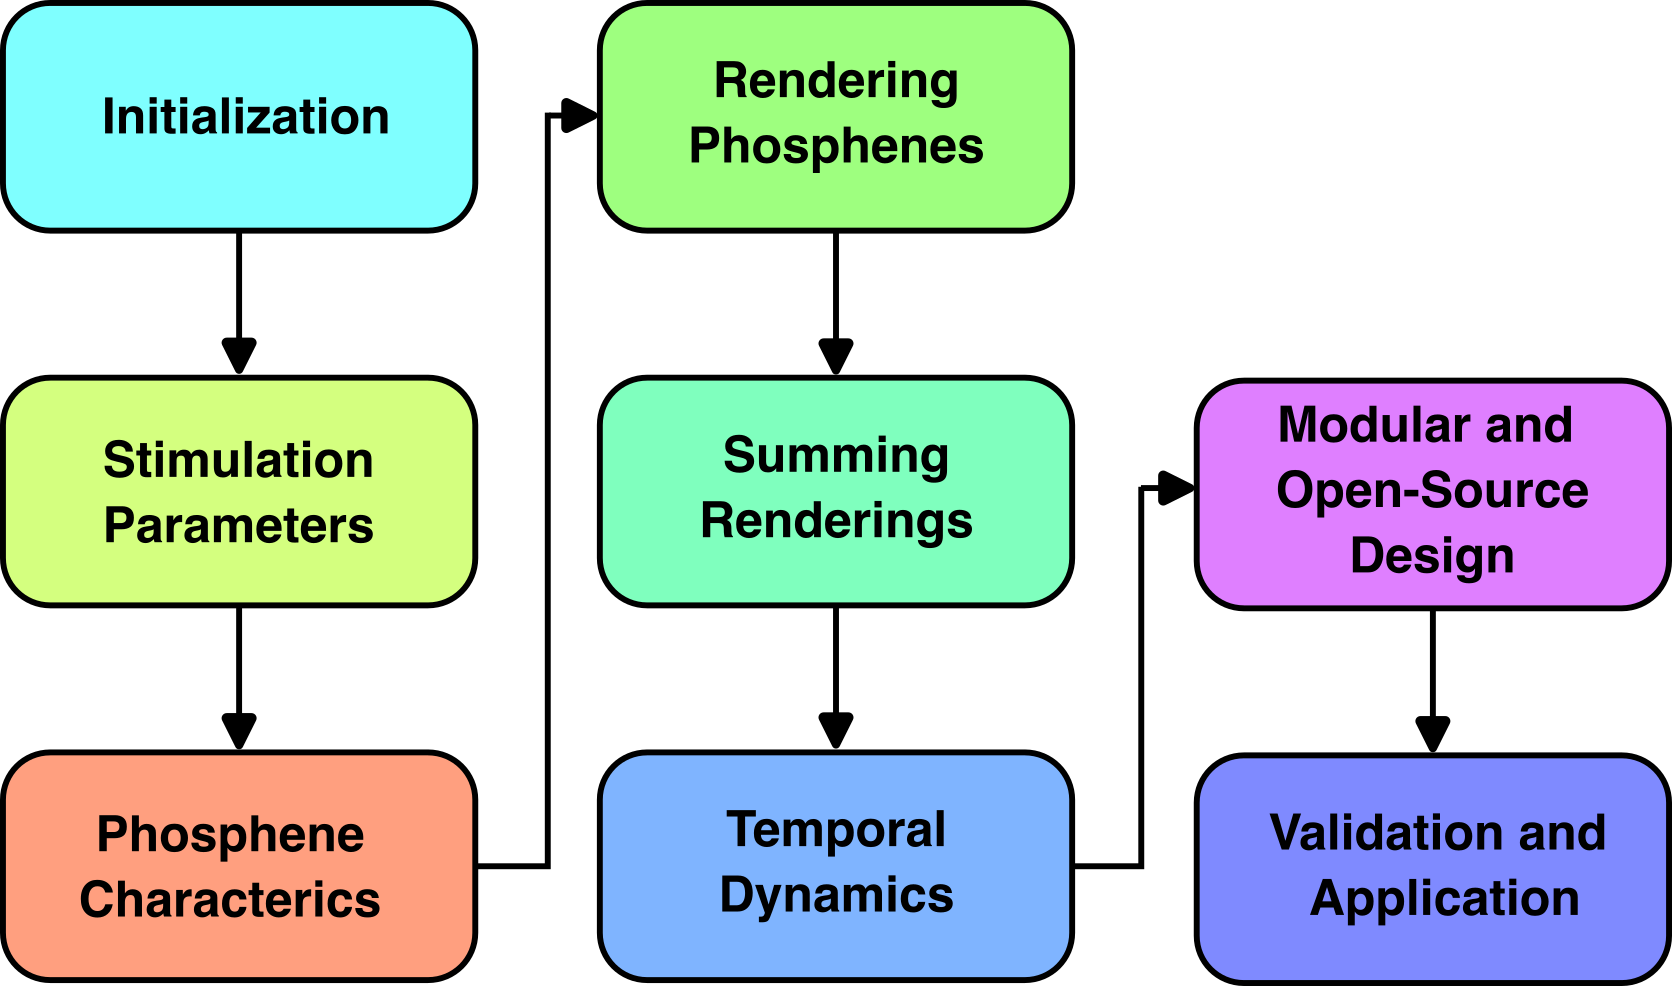
\includegraphics[width=0.6\textwidth]{imgs/block_diagram_vis_prost.png}
  \caption{| Overview of a Visual Prosthesis Simulation Framework. The
    simulator is initialized with electrode locations on a visuotopic
    map of the visual cortex (V1), representing the spatial organization
    of the visual field. For each frame, it processes stimulation
    parameters such as amplitude, pulse width, and frequency for each
    electrode. Using these parameters and electrode locations, it
    estimates phosphene characteristics, which are rendered on a visual
    field map considering cortical magnification and activation
    thresholds. Individual phosphene renderings are summed to produce
    the simulated prosthetic percept. Temporal dynamics, including
    delayed onset and offset of perception, are modeled using a leaky
    integrator. The simulator's modular and open-source design,
    implemented in Python with PyTorch for example, allows for fast GPU
    computations and easy integration with external
    software~\parencite{deruytervansteveninckEndtoendOptimizationProsthetic2022}.
    It is validated through computational and behavioral experiments,
    incorporating neurophysiological and clinical findings to ensure
    biological plausibility.}\label{fig:simulator_framework}
\end{figure*}

Deep learning can enhance these simulators by integrating them into end-to-end
optimization pipelines. In such systems, a Convolutional Neural Networks (CNN)
can be used to process input images or video frames and generate appropriate
electrical stimulation parameters. The simulator then creates a visual
representation based on these parameters, which another CNN evaluates by
attempting to reconstruct the original input image. The entire system is trained
through backpropagation, where the error in the reconstructed image is used to
update the parameters of the networks, optimizing the stimulation parameters for
better visual perception.

This deep learning approach allows for the dynamic optimization of stimulation
patterns, potentially improving the quality and functionality of prosthetic
vision. It enables the simulator to adapt to complex visual stimuli and optimize
the information encoded in the phosphenes, making the simulated vision more
useful for real-life applications. As this technology is rather experimental
still, most of the research is still being done in controlled environments with
virtual reality headsets that are able to adequately simulate phosphene vision
for testing.

However, the current simulator is limited to static images due to scene
simplification and limited textures on object. The simulator also does not account for the temporal dynamics of real-world
environments. Furthermore, the resolutions of phosphenes are still limited even
under constant light intensity, which is much more varied in real scenario's. To
address this issue, new models must be developed that can process video streams
and generate appropriate stimulation patterns in real-time. Different models for
image pre-processing of different situations should be able to adapt to changes
in the visual scene, ensuring that the user receives accurate and up-to-date
information about their surroundings.

\section*{Research}\label{sec:research}
\subsection*{Objective}\label{subsec:objective}
This study aims to develop a novel approach to generating phosphene patterns in
a way that dynamics environments can be visualized in real-time. These dynamic
systems as of yet, do not exist and are crucial for the development of visual
aid systems that can adapt to more complex and real-world scenarios. If
successful, these improved prosthetic systems hold potential of increasing the
blind user's experience dramatically.

To advance the development of visual cortical prostheses, the first step
involves creating and testing initial AI algorithms aimed at simplifying scenes
and generating phosphene patterns. This will include leveraging deep learning
techniques, such as Convolutional Neural Networks (CNNs), to process complex
visual inputs and translate them into simplified phosphene representations.
These algorithms will focus on maintaining essential visual information while
reducing complexity to ensure that the generated phosphene patterns are
interpretable and useful for the user.

Simultaneously, the experimental infrastructure will be established to support
this research. This infrastructure will encompass the necessary hardware and
software setups, including high-performance computing systems equipped with GPUs
for running deep learning models and the phosphene simulator. Additionally, a
controlled environment for conducting experiments with both simulated and real
participants will be developed, ensuring accurate data collection and analysis.
This foundational setup will enable rigorous testing and refinement of the AI
algorithms, facilitating the progression toward functional and practical visual
prosthetic systems.

\subsection*{Approach}\label{subsec:approach}
\todo[inline]{Be more concrete and add references to valid techniques where necessary.}
\subsubsection*{Phase 1: AI Algorithm Development and Initial Testing}
In the initial phase of this research, the primary objectives are to develop and
test AI algorithms designed for scene simplification and phosphene pattern
generation, as well as to establish the experimental infrastructure necessary
for subsequent studies. To achieve these goals, a diverse group of 20
participants, all without visual impairments, will be recruited to participate
in a series of experiments. These participants will navigate indoor courses of
varying complexity and dynamic elements while wearing VR headsets integrated
with an adaptive scene simplification system. The experiments will be conducted
under three distinct conditions: a fixed scene simplification as the baseline,
an adaptive scene simplification utilizing the newly developed AI algorithm, and
an adaptive scene simplification with multi-modal feedback that includes both
haptic and auditory cues. Throughout these trials, data will be collected on
trial duration, the number of collisions, subjective difficulty ratings, and
qualitative feedback from participants. This phase aims to refine the initial AI
models and ensure that the experimental setup is capable of providing reliable
and accurate data, thus laying a solid foundation for the subsequent phases of
the research.

\subsubsection*{Phase 2: Advanced AI and Neurophysiological Studies}
The second phase of the research focuses on implementing and testing advanced AI
algorithms alongside conducting neurophysiological studies to assess their
impact on visual perception. This phase involves developing more sophisticated
AI models, including Convolutional Neural Networks (CNNs), Generative
Adversarial Networks (GANs), and Reinforcement Learning (RL) algorithms, with an
emphasis on integrating edge computing for real-time processing. The
neurophysiological component of this phase will utilize Visual Evoked Potentials
(VEP) and functional near-infrared spectroscopy (fNIRS) to study the effects of
the adaptive systems on visual perception. Participants will engage in tasks
such as navigation, object recognition, and reading, with performance metrics
including accuracy, response time, error rate, and trial duration, in addition
to neurophysiological data. By correlating these metrics with neurophysiological
responses, this phase aims to provide a deeper understanding of how advanced
AI-driven systems influence visual processing, thereby guiding further
refinements and improvements.

\subsubsection*{Phase 3: Full-scale Experiments and Final Analysis}
The final phase of the research involves conducting extensive behavioral and
neurophysiological experiments with larger participant groups to validate the
effectiveness and reliability of the developed AI systems. This phase will
encompass a comprehensive set of behavioral experiments designed to collect
extensive performance data from a larger cohort, thereby enabling a robust
evaluation of the system's efficacy in diverse real-world scenarios.
Concurrently, neurophysiological studies will continue with an expanded
participant group to ensure the generalizability of the findings. Detailed
analysis of patterns and insights derived from the collected data will be
performed to fine-tune the AI models and validate the improvements made
throughout the research. The ultimate aim of this phase is to ensure that the
AI-driven visual prosthetic system is ready for real-world application,
significantly enhancing the visual experiences of users with visual impairments
and contributing valuable knowledge to the field of neuroprosthetics.

\section*{Innovation}\label{sec:innovation}
\subsection*{AI-Enhanced Visual Prostheses}
The proposed research is pioneering in its integration of advanced artificial intelligence (AI) and virtual reality (VR) to develop and enhance visual prostheses. This innovative approach leverages state-of-the-art deep learning algorithms, such as Convolutional Neural Networks (CNNs), Generative Adversarial Networks (GANs), and Reinforcement Learning (RL), to process complex visual inputs and generate simplified phosphene patterns that are interpretable and useful for users. By embedding these AI algorithms within a VR environment, the system can dynamically adapt to changes in the visual scene, thereby providing real-time scene simplification and improving the responsiveness of the prosthetic device. This integration is expected to significantly enhance the user experience, offering more accurate and detailed visual representations that are crucial for navigating dynamic and complex environments. The incorporation of multi-modal feedback, including haptic and auditory cues, further enhances the system's ability to provide comprehensive sensory information, thus creating a more immersive and effective visual aid.

\subsection*{Real-world Applications}
The potential real-world applications of this research are profound,
particularly in terms of improving the quality of life for individuals with
severe visual impairments. By enabling these individuals to perceive their
surroundings more clearly and respond more effectively to dynamic changes, the
developed system can facilitate greater independence and confidence in daily
activities. The anticipated improvements in scene simplification and
responsiveness are not only expected to enhance basic navigation and object
recognition but also to support more complex tasks such as reading and social
interactions. Beyond the immediate benefits to end-users, this research has
broader implications for the field of neuroprosthetics and adaptive technology.
It demonstrates the feasibility and advantages of integrating AI and VR to
create more sophisticated and adaptive prosthetic devices, setting a new
standard for future developments. Moreover, the insights gained from this
research could inform the design and implementation of other types of neural
interfaces, potentially leading to advancements in treating various neurological
conditions and enhancing sensory augmentation devices. This project stands at
the forefront of a transformative shift in how technology can be harnessed to
improve human capabilities and overall well-being.
\todo[inline]{Maybe add some information on potential clinical applications.}

\section*{Future Impact}\label{sec:impact}
\subsection*{Contribution to the Field}
This research is poised to make significant contributions to the field of visual
cortical prostheses by advancing the integration of artificial intelligence (AI)
and virtual reality (VR) systems in developing adaptive visual aids. The
innovative AI algorithms and real-time processing capabilities proposed in this
study are expected to enhance the functionality and usability of visual
prostheses, offering more accurate and dynamic visual representations for users.
These advancements will address current limitations in phosphene resolution and
scene simplification, potentially transforming how visual information is
processed and perceived by individuals with visual impairments. Moreover, the
successful implementation of these technological advancements could pave the way
for future research and development in related areas, such as the optimization
of other neural interfaces and sensory augmentation devices. The insights gained
from this study will provide a valuable foundation for further exploration into
AI-enhanced neuroprosthetics, encouraging ongoing innovation and improvement in
this critical field.

\subsection*{Call to Action}
The importance of continued interdisciplinary research cannot be overstated in
the quest to advance visual prosthesis technology. This proposal underscores the
need for collaboration between neuroscience, engineering, and AI to fully
realize the potential of these groundbreaking elements in technological
possibility. By fostering partnerships across these disciplines, we can
accelerate the development of more effective and sophisticated visual aids,
ultimately improving the quality of life for individuals with severe visual
impairments. We encourage researchers, practitioners, and stakeholders in these
fields to work together, share knowledge, and contribute to the collective
effort to enhance neuroprosthetic devices. The future of visual cortical
prostheses depends on our ability to integrate diverse expertise and innovate at
the intersection of these dynamic and rapidly evolving fields.

\section*{Timetable}\label{sec:timetable}
The Gannt-chart goes here with a brief explanation of the different phases.
\todo[inline]{Add a Gannt-chart with the different phases and milestones based on the word document containg the time phases.}
\printbibliography%

\section*{Rebuttal}\label{sec:rebuttal}
After the first review of the draft, the proposal was revised to address the
reviewers' comments. The main changes are listed below:

\todo[inline]{Add rebuttal comments here after 1st review.}

\end{document}